\documentclass[12pt]{article}
\usepackage{graphicx}
\graphicspath{ {./images/} }
\usepackage{amsthm,amssymb,amsmath,amsfonts}
\usepackage[a4paper, top=25mm, bottom=30mm, left=25mm, right=25mm]{geometry}
\usepackage[pagebackref=false,colorlinks,linkcolor=black,citecolor=black]{hyperref}
\usepackage[nameinlink]{cleveref}
 \AtBeginDocument{%
    \crefname{equation}{برابری}{equations}%
    \crefname{chapter}{فصل}{chapters}%
    \crefname{section}{بخش}{sections}%
    \crefname{appendix}{پیوست}{appendices}%
    \crefname{enumi}{مورد}{items}%
    \crefname{footnote}{زیرنویس}{footnotes}%
    \crefname{figure}{شکل}{figures}%
    \crefname{table}{جدول}{tables}%
    \crefname{theorem}{قضیه}{theorems}%
    \crefname{lemma}{لم}{lemmas}%
    \crefname{corollary}{نتیجه}{corollaries}%
    \crefname{proposition}{گزاره}{propositions}%
    \crefname{definition}{تعریف}{definitions}%
    \crefname{result}{نتیجه}{results}%
    \crefname{example}{مثال}{examples}%
    \crefname{remark}{نکته}{remarks}%
    \crefname{note}{یادداشت}{notes}%
    \crefname{observation}{مشاهده}{observations}%
    \crefname{algorithm}{الگوریتم}{algorithms}%
    \crefname{cproof}{برهان}{cproofs}%
}

\usepackage{tikz}
\usepackage{graphicx}
\usepackage{color}

\usepackage{setspace}
\doublespacing

\usepackage{titletoc}
\usepackage{tocloft}
\usepackage{enumitem}

\usepackage{algorithm}
% \usepackage[noend]{algpseudocode}
\usepackage[noend]{algorithmic}
\renewcommand{\algorithmicrequire}{\textbf{Input:}}
\renewcommand{\algorithmicensure}{\textbf{Output:}}

\usepackage{tabularx}
\makeatletter
\newcommand{\multiline}[1]{%
  \begin{tabularx}{\dimexpr\linewidth-\ALG@thistlm}[t]{@{}X@{}}
    #1
  \end{tabularx}
}
\makeatother

\usepackage{float}
\usepackage{verbatim}
\makeindex
\usepackage{sectsty}
\usepackage{xepersian}
\SepMark{-}
\settextfont[Scale=1.2,Path=fonts/,BoldFont=B Nazanin Bold.ttf]{B Nazanin.ttf}
\setlatintextfont{Times New Roman}
\renewcommand{\labelitemi}{$\bullet$}

\theoremstyle{definition}
\newtheorem{definition}{تعریف}[section]
\newtheorem{remark}[definition]{نکته}
\newtheorem{note}[definition]{یادداشت}
\newtheorem{example}[definition]{نمونه}
\newtheorem{question}[definition]{سوال}
\newtheorem{remember}[definition]{یاداوری}
\newtheorem{observation}[definition]{مشاهده}
\theoremstyle{theorem}
\newtheorem{theorem}[definition]{قضیه}
\newtheorem{lemma}[definition]{لم}
\newtheorem{proposition}[definition]{گزاره}
\newtheorem{corollary}[definition]{نتیجه}
\newtheorem*{cproof}{برهان}




\begin{document}
\fontsize{12pt}{14pt}\selectfont
\begin{minipage}{0.1\textwidth}

\end{minipage}%
\hfill%
\begin{minipage}{0.6\textwidth}\centering
\fontsize{10pt}{10pt}\selectfont
به نام خداوند \\
تئوری یادگیری ماشین \\
دکتر سیدصالحی\\
جلسه سوم
 \\
\vspace{0.25cm}
\begingroup
\fontsize{8pt}{8pt}\selectfont
دانشکده ریاضی و علوم کامپیوتر \\
اسفند ماه 1402\\
\endgroup
\end{minipage}%
\hfill%
\begin{minipage}{0.1\textwidth}
\end{minipage}

\vspace{0.5cm}

\noindent\rule{\textwidth}{1pt}

\section*{مسئله یادگیری}
یادگیری فرآیند ایجاد تعمیم از داده های $noisy$ است. این شامل $abstraction$ برای تفسیر داده ها، پیاده سازی برای کاربرد نتایج یادگیری و ارزیابی برای اصلاح درک و بهبود نتایج.
\\
\subsection*{مثالی از مسئله یادگیری ماشین(پیش بینی خطر حمله قلبی)}
مسئله ای که اینجا هست بدست آوردن ریسک خطر حمله قلبی بر اساس دیتا موجود است. یادگیری ماشین می تواند برای پیش بینی خطر حمله قلبی استفاده شود. این کار را با شناسایی الگوهایی در داده‌ها انجام می‌دهد که ممکن است از نظر ریاضی قادر به شناسایی آنها نباشیم.

\begin{figure}[htbp]
    \centering
    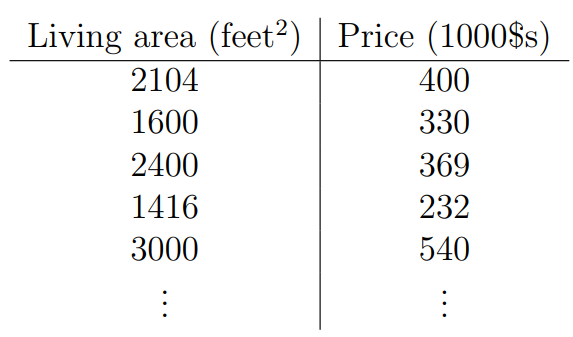
\includegraphics[width=0.6\textwidth]{etc/Images/Fig1.png}
    \caption{جدول سن، جنسیت، وزن و وضعیت دیابت یک فرد و اینکه آیا ریسک خطر حمله قلبی وجود دارد یا خیر را نشان میدهد.}
    \label{Fig1}
\end{figure}
\\

\subsection*{اجزای یادگیری}
\begin{enumerate}
  \item تابع هدف ناشناخته: این تابع که با $t$ نشان داده می شود، ورودی $x$ را به خروجی $y$ نگاشت می کند. هدف از یادگیری، تقریب زدن این تابع ناشناخته است.
  \item مثال‌های آموزشی: اینها جفت هایی از داده‌ ها هستند $(x,y)$، که الگوریتم یادگیری به آنها دسترسی دارد. هر مثال آموزشی نشان دهنده یک رابطه ورودی-خروجی واحد است.
  \item الگوریتم یادگیری: این الگوریتمی است که نمونه های آموزشی را به عنوان ورودی می گیرد و یک فرضیه را که تقریبی از تابع هدف ناشناخته است را از میان فرضیه ها موجود، خروجی می دهد.
  \item فرضیه نهایی: این تقریب تابع هدف مجهولی است که الگوریتم یادگیری تولید کرده است. با $g$ نشان داده می شود و عنصری از مجموعه فرضیه است که با $H$ نشان داده می شود.
\end{enumerate}

\begin{figure}[htbp]
    \centering
    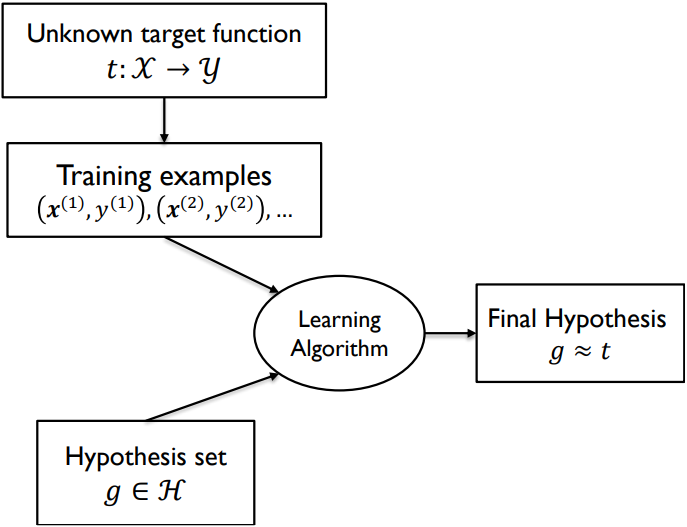
\includegraphics[width=0.7\textwidth]{etc/Images/Fig2.png}
    \caption{نمودار پنج جزء یادگیری را نشان می دهد.}
    \label{Fig2}
\end{figure}

مؤلفه کلیدی مدل یادگیری است که از مجموعه ای از فرضیه ها تشکیل شده است. از این فرضیه ها برای تخمین مقدار یک تابع هدف استفاده می شود که ناشناخته است. الگوریتم یادگیری برای جستجو در میان مجموعه فرضیه ها و یافتن فرضیه ای که به بهترین وجه تابع هدف را تقریب می کند، استفاده می شود. این کار با استفاده از مثال های آموزشی که جفت مقادیر ورودی و خروجی هستند انجام می شود. سپس الگوریتم یادگیری از این مثال‌ها تعمیم می‌یابد تا در مورد داده‌های جدید و دیده نشده پیش‌بینی کند.

\subsection*{ادامه مثال}
میتوان ویژگی های یک فرد را به عنوان یک بردار ورودی نشان داد، از جمله سن، جنسیت، وزن، و اینکه آیا دیابت دارد یا خیر و اینکه آیا فرد در خطر حمله قلبی قرار دارد یا خیر.

\begin{figure}[htbp]
    \centering
    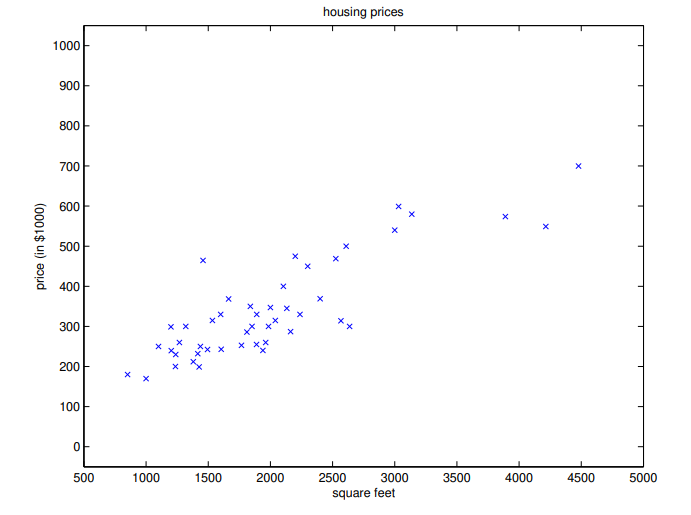
\includegraphics[width=0.7\textwidth]{etc/Images/Fig3.png}
    \caption{جدول سن، جنسيت، وزن و وضعيت ديابت يك فرد و اينكه آيا ريسك خطر حمله قلبي وجود دارد يا خير را نشان ميدهد را میتوان پارامتری کرد و به عنوان بردار ورودی داد.}
    \label{Fig3}
\end{figure}

پرسپترون ها نوعی $classifier$ خطی هستند که می توانند برای پیش بینی های دودویی استفاده شوند. اگر مجموع وزنی بیشتر از یک $threshold$ ای باشد، خروجی پرسپترون 1 است. در غیر این صورت، 0 را خروجی می دهد. در این مثال، پرسپترون از ویژگی های فرد برای پیش بینی اینکه آیا در معرض خطر حمله قلبی است یا خیر استفاده می کند.
\\
توجه به این نکته مهم است که این یک مثال ساده شده است و مدل‌های پیچیده‌تر معمولاً در عمل برای پیش‌بینی خطر حمله قلبی استفاده می‌شوند.
\\
\\
میتوان یک شخص در معرض خطر را به صورت زیر در تعریف بالا را نوشت:
\[
\sum_{i=1}^{d}w_{i}x_{i}>threshold
\]

تابع فرضیه الگوریتم یادگیری پرسپترون ($PLA$) را نیز به شکل زیر نشان میدهیم:
\[
h(x) = \sum_{i=1}^d sign(w_i x_i - threshold)
\]
\[
sign(x) = \begin{cases}
+1, & if  x \geq 0 \\
-1, & if  x < 0
\end{cases}
\]

\\
\\
هدف این است که جعبه ای بسازیم که بتواند خروجی صحیح $y_i$ را زمانی که ورودی $x_i$ داده می شود تولید کند. ذخیره سازی داده ها و نتایج در یک جدول دو چالش اصلی را به همراه دارد: اولاً، یک ورودی ممکن است با خروجی های متعدد در جدول مطابقت داشته باشد، و ثانیاً، گنجاندن داده های ورودی جدید می تواند مشکل ساز باشد. از این رو، ما به دنبال پرداختن به این مسائل از طریق ترکیبی از تعمیم و حفظ کردن، با درونیابی به عنوان راه حل پیشنهادی هستیم.


\subsection*{پارادایم های یادگیری ماشین}
سه پارادایم اصلی یادگیری ماشین وجود دارد: یادگیری $supervised$، یادگیری $unsupervised$ و $learning$ $reinforcement$.

\begin{itemize}
    \item یادگیری $supervised$ نوعی از یادگیری ماشین است که در آن یک مدل با استفاده از داده های $lable$ شده آموزش داده می شود. داده های $lable$ شده شامل داده های ورودی و خروجی مورد نظر مربوطه است. مدل یاد می گیرد که داده های ورودی را به خروجی مورد نظر نگاشت کند. به عنوان مثال، یک مدل یادگیری نظارت شده می تواند برای پیش بینی قیمت یک خانه با توجه به اندازه، مکان و سایر ویژگی های آن آموزش ببیند.
    \item یادگیری $unsupervised$ نوعی از یادگیری ماشین است که در آن یک مدل با استفاده از داده های بدون $lable$ آموزش داده می شود. داده های بدون $lable$ فقط از داده های ورودی تشکیل شده است، بدون هیچ $lable$ مربوطه. مدل یاد می گیرد که الگوها یا ساختارها را در داده ها پیدا کند. برای مثال، می‌توان از یک مدل یادگیری بدون نظارت برای دسته‌بندی مشتریان در گروه‌های مختلف بر اساس سابقه خریدشان استفاده کرد.
    \item $learning$ $reinforcement$ نوعی از یادگیری ماشین است که در آن یک مدل از طریق آزمون و خطا یاد می گیرد. مدل با یک محیط تعامل می کند، اقداماتی انجام می دهد و بر اساس نتیجه اقدامات خود پاداش یا جریمه دریافت می کند. مدل یاد می گیرد که اقداماتی را انجام دهد که پاداش آن را به حداکثر می رساند. به عنوان مثال، یک مدل یادگیری تقویتی می تواند برای آموزش راه رفتن یک ربات با پاداش دادن به ربات برای برداشتن گام هایی در جهت درست استفاده شود.
    \\
    \\
    یک $agent$ در $learning$ $reinforcement$ باید با دنیای خود تعامل داشته باشد و از این طریق بیاموزد که چگونه مقداری پاداش تجمعی را در طول زمان به حداکثر برساند.
    
\end{itemize}

همچنین پارادایم های دیگری از یادگیری ماشینی مانند یادگیری $semi-supervised$، $learning$ $online$ و $learning$ $active$ اشاره می کند. این پارادایم ها تغییراتی از سه پارادایم اصلی مورد بحث در بالا هستند.

\subsubsection*{مثال یادگیری $supervised$}
پروتئین‌ها، متشکل از 20 اسید آمینه استاندارد، اساساً به‌عنوان زبانی با الفبای 20 حرفی خود عمل می‌کنند، جایی که توالی‌های مختلف $functionality$ های متفاوتی را ارائه می‌دهند. چالش در نگاشت دقیق این توالی ها به $functionality$ های مربوطه نهفته است. با این حال، آزمایش عملی برای دستیابی به این نقشه برداری به دلیل هزینه های بالای آن مانع می شود. در حالی که داده های قابل توجهی در مورد این نگاشت ها وجود دارد، تخمین زده می شود که کمتر از 10 درصد تا کنون شناسایی شده است. در نتیجه، اکثر نگاشت ها نا پیدا باقی می‌مانند. با این وجود، به نظر می‌رسد یک الگوی قابل تشخیص در نگاشت‌های شناسایی‌شده وجود دارد که کاربرد بالقوه تکنیک‌های یادگیری $supervised$ را پیشنهاد می‌کند.

\begin{figure}[htbp]
    \centering
    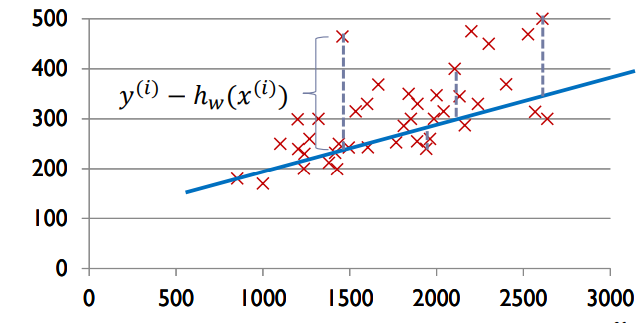
\includegraphics[width=0.7\textwidth]{etc/Images/Fig4.png}
    \caption{یک $illustration$ از رشته ای آمینو اسید ها.}
    \label{Fig4}
\end{figure}


\end{document}